\documentclass[12pt,oneline,a4paper,numbib]{ouparticle}
\usepackage{array,multirow,graphicx}
\usepackage{pdflscape}% for landscape

\usepackage{adjustbox}     % adjusting table (too wide)
\usepackage{rotating}      % sidewaytables
\usepackage{array}
\usepackage{stackengine}

\usepackage{amsmath} % \numberwithin{equation} doesn't exist without this package.
\numberwithin{equation}{subsection} % This line resets equation numbering when starting a new section.
\renewcommand{\theequation}{Eq. \thesubsection.\arabic{equation}} % This line ads "Eq." in front of your equation numbering.

\begin{document}

\title{MSE and dynamic state variable model with sigma function}

\author{%
\name{Nekane Alzorriz}
\address{European Commission, Joint Research Centre (JRC), Sustainable Resources Directorate, Water and Marine Resources Unit, Via Enrico Fermi 2749, 21027 Ispra, Italy.}
\email{nekane.alzorriz@gmail.com}
\and
\name{Jan Jaap Poos}
\address{Wageningen Marine Research, PO Box 68, 1970 AB IJmuiden, The Netherlands.}
\email{janjaap.poos@wur.nl}}

\abstract{
TBD
We contrast three types of management plans to achieve maximum sustainable yields (MSY) from multiple stocks and compare their effectiveness based on a management strategy evaluation (MSE) that uses a dynamic state variable model including errors in decision-making in its operating model.}

\date{\today}

\keywords{management stategy evaluation; dynamics state variable model; errors in decision-making; landing obligation; maximum sustainable yield}

\maketitle


\section{Introduction}


We have to make sure we are clear on the ages of the species: do we start at 0 or at 1?

Management strategy evaluation (MSE; \cite{Bunnefeld2011, Sainsbury2000, Smith1994}) seeks to study the implications of management strategies using simulation\cite{Punt2016}. Such simulation should include all important processes of a fishery, which is inherently a socio-ecological system, with coupled dynamics of the fishing fleets, the exploited stocks, and their governance\cite{Punt2016,Rasemeyer2007}. Given the complexity of such a socio-ecological system the uncertainy about the dynamics and feedbacks are consideable. As a result, any forecasted success in achieving goals in a management strategy may thus be inperceivably small compared to the stochasticity in results generated in the system, or worse, be counteracted by unintended consequences of the management strategy. The robustness of management strategies to the uncertainy in the processes that govern fisheries systems thus need to be accounted for \cite{Andersen2010, Kell2007, Prellezo2016, Punt2016}. 

The adaptive response of fishers to their environment is one of the key uncertainties requiring attention in MSE \cite{Fulton2007}. Simulation tools for such adaptive responses are available in fisheries, borrowing methodology from the more general question of state-dependent foraging decisions in ecological systems \cite{ClarkandMangel2000,Houston1999}. New tools for state-dependent behaviour of individual fishing vessels, translated into behaviour of the fleet and implemented using stochastic dynamic programming \cite{Alzorriz2018,Batsleer2015, Dowling2011, Poos2010, Gillis1995} have been developed. These models generally predict the effect in the short term (within a fishing trip, or a quota year) by optimizing a utility function and determine which choices best yields the best chance of increasing utility, while keeping track of the state of each individual. The effect of a choice on the utility depends on the economic environment, such as the home port of the vessel and the distance to fishing grounds, and the biological enviroment, such as the spatial distribution of the resources. Using such dynamic variable state models, effects of e.g. relocation costs of marine protected areas have been modelled \cite{Dowling2011}.

Dynamic state variables have also been used to describe discarding behaviour \cite{Batsleer2015, Batsleer2013, Gillis1995}. These studies may shed light on the potential outcomes of the European fisheries management reform of 2013. That reform included using the use of the Maximum Sustainable Yield (MSY) reference points as targets for exploiting commericially important fish stocks and the gradual introduction of a landings obligation (LO) \cite{CFP2013}. Indeed, using spatial and temporal distributions of catch rates within a single year, dynamic state variable models forecasted  high costs in mixed fisheries in the short term as a result of the LO. These costs result from removing the option to adapt landings to quota by discarding parts of the catch \cite{Alzorriz2018}. This will result in fishing effort reallocation and early closures of fisheries once quota have been reached. However, the  long term benefits to fisheries that could result from improved selectivity are ignored in those studies. Ignoring the potential for improved selectivity leaves out a key element in the perceived benefit of the LO. Because the LO should provide incentives for the use of more selective gears and for fisheries to  move away from areas with high levels of unwanted catch \cite{Alzorriz2016, Alzorriz2018}, the improved selectivity should lead to higher long term catches. Achieving single species MSY while landing all commercial catches in fisheries targeting multiple species (mixed fisheries) is challenging because achieving the objective for one species may mean missing the objective for another \cite{Batsleer2013,Ulrich2017}. Forecasting whether such management will be effective depends on understanding the response of individual effort allocation to the management.

To enable longer term prediction of the effects of changes in fisheries management, and thus complete the Management Strategy Evaluation, one needs to couple the fleet dynamic models that forecast the fleet response to management to  biological dynamic models that forecast the fish population responses to the changing fleet response. We present an MSE that encompasses the individual harvester decision-making process and socioeconomic drivers on management effectiveness, i.e. if the fleet dynamic model results in a short term movement of vessels to allocate effort both spatially and temporally, we also expect longer term changes to occur in fish populations and the economy of the fishery \cite{Alzorriz2018}. Such combination needs to be responsive to all the drivers that influence and motivate the actual fleet and to respect existing constraints \cite{Venables2009}. The drivers will include the (real or perceived) local abundance and catchability of the fished stocks and various resource costs, principally that of fuel. The constraints will include the obvious management-imposed constraints such as levels of total allowable catch, and economical constraints such as the contribution of the annual fines for exceeding catch quotas.

Using a MSE, the main objective of this work is not to reproduce the entire complexity of a real mixed fishery, but to defined plausible hypothesis about population dynamics and then to implemented the processes of interest, i.e., changes in population abundance, to finally measure the effect of the potential consequences associated with the fishers optimal choice location underlying assumption of the current state-dependent behaviour of individual fishing vessels. To understand the fleet dynamics in a spatially and temporally heterogeneous mixed quota-regulated fishery when reducing from unmanaged (unconstrained catch quota) to MSY managed and to compare it with a situation where discards are allowed in order to assess on the biological and economic consequences. If LO and catch quotas are not fully enforced, there will be an incentive to continue discarding. Therefore, this manuscript tends to understand the likely adaptive change in fishing patterns that will help us to understand if this leads to a better balance between quotas and catches.

%Since maximizing effort does not maximize catch, the question is if there is an optimum fishing rate that would lead to a maximum yield.


\section{Methods}


The Managament Strategy Evaluation framework was used to forecast the dynamics of a hypothetical mixed fishery on two species. The framework consists of an Operating Model (OM) and a Management Procedure (MP). In the fishery, there are three essential elements: (i) a collection of size strucured fish stocks, whose dynamics are governed by annual reproduction, growth, migration, and mortality. (ii) A management body that evaluates the fishing pressure and aims to set annual quotas in accordance with fishing mortalities dictated by FMSY reference points. (iii) a fleet of individual fishers who aim to make the best use of their annual quota. Within this mixed fishery, individual vessels make adaptive choices on fishing location and discarding that depend on the distribution of the resources, and the quota that they are allocated. Each of these elements is discussed in more detail below. The essential elements of the framework are summarized in Figure \ref{fig:MSE}.

The OM captured the key processes in the dynamics of the fish populations, the fisheries and the management body, and can be thought of as a minimum realistic model \cite{Punt1995}.  The operating model thus includes  individual harvester decision-making (including error) and the consequent biomass of fish stocks, including the essential elements for calculating the individual harvester economic performance. The  management body used the MP to make its decision on how to respond to the state of the resource  (Figure \ref{fig:stockdyn}). This management procedure thus includes the data collection from the fishery, how these are interpreted, and the Harvest Control Rule that dictates the limits that are set to the fishery. 

 
\begin{figure}[!h]
\centering
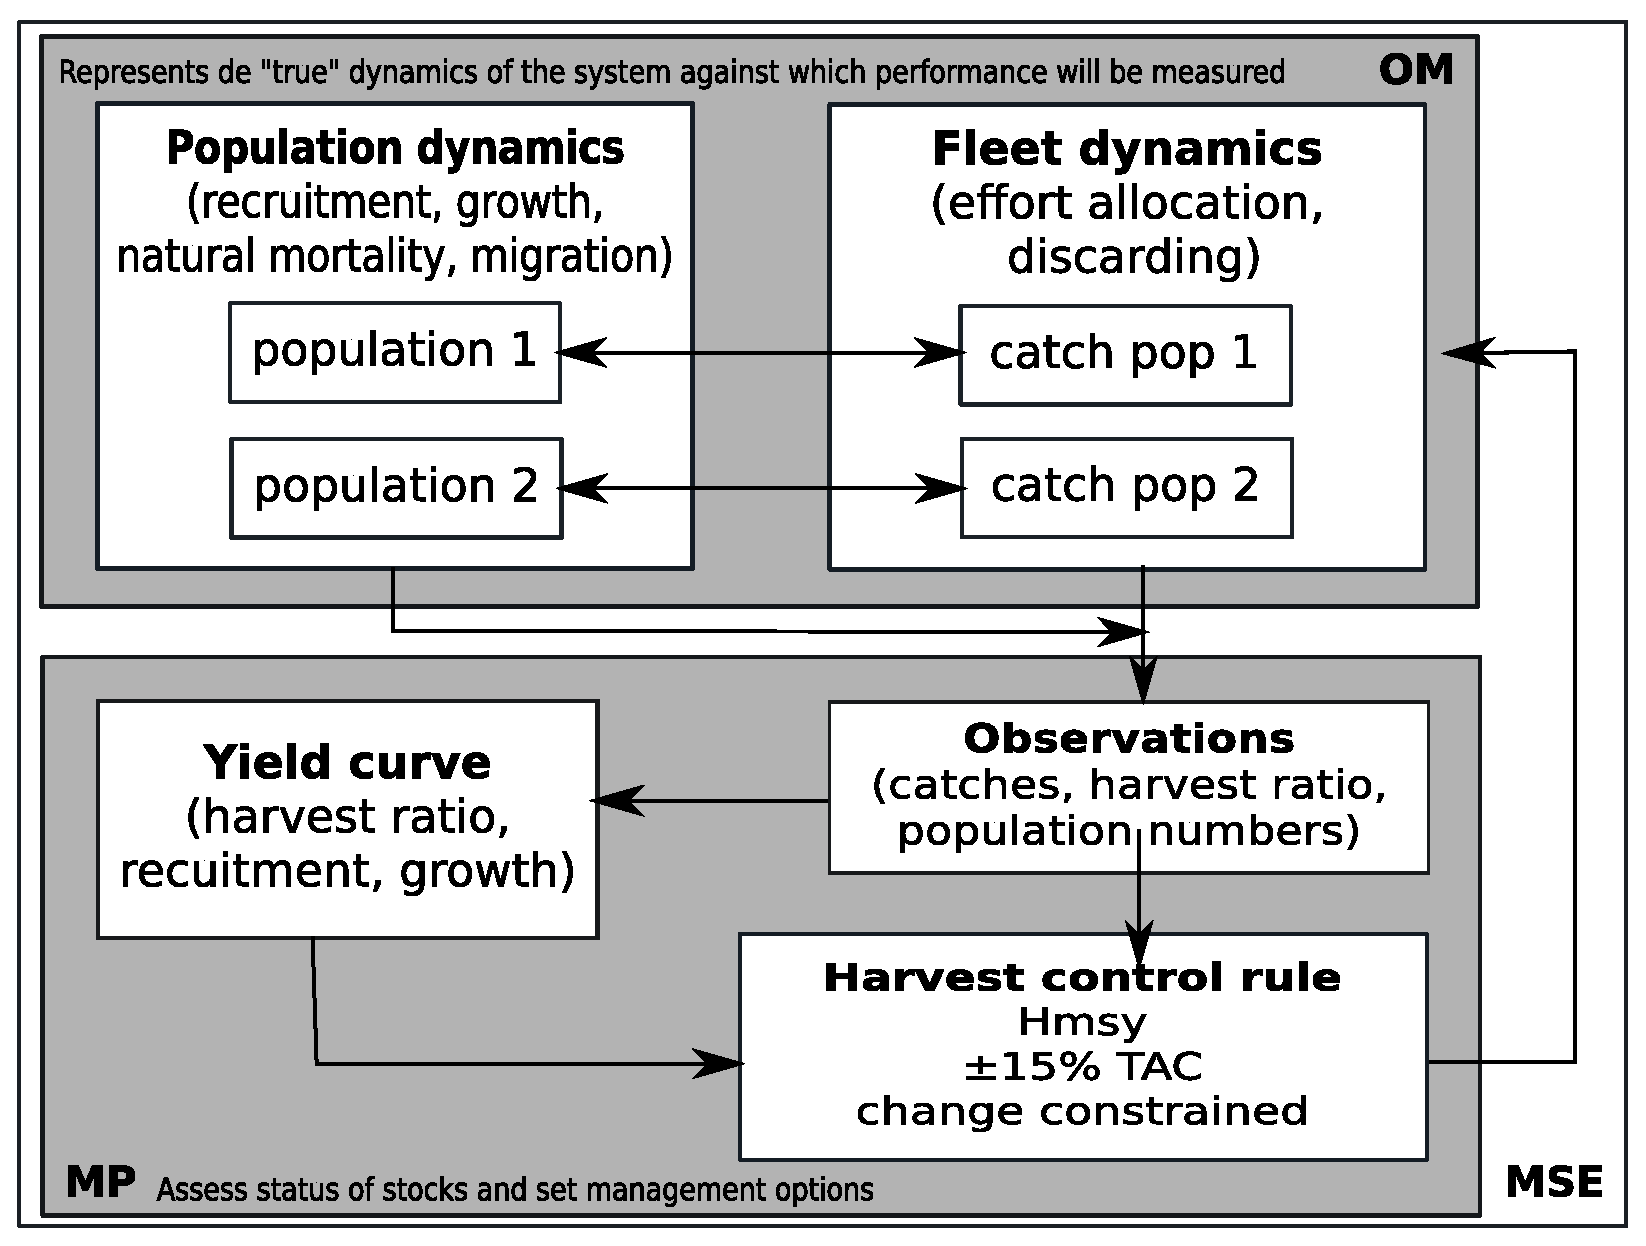
\includegraphics[width=0.55\textwidth]{Figures/MSE.eps} 
\caption{Conceptual overview of the Managament Strategy Evaluation approach, including the Operating Model (OM) and the Management Procedure (MP) components of the framework.}
\label{fig:MSE}
\end{figure}

\begin{figure}[!h]
\centering
\includegraphics[width=0.4\textwidth]{Figures/Areadynamics.eps} 
\caption{The Operating Model (OM) component, including the key processes in the dynamics of the fish populations.}
\label{fig:stockdyn}
\end{figure}

\subsection{Population dynamics}


To allow the fishery to make spatial and temporal choices, the model needed to be seasonally and spatially explicit. The dynamics of the fish stocks were modelled using an age-structured model that was spatially explicit, with seasonal time steps. In each seasonal time step, fish grow, migrate, and die. The number of fish of stock $i$ of age $a$ at year $y$, in season $s$, and area $p$ was written as $N_i (a, y, s, p)$.  The ages in the model range between age 0 and age $A$, the maximum age in the model. The seasons range between season 1 and season $S$, the last season within each year. Individuals were born at age 0, at the start of each year $y$, in season 1. The number of new-born individuals $R_i (p)$ in the model was a function of the area $p$ and independent of the size of the adult population. The population numbers at age 0 are thus
 
\begin{equation}
N_i (0, y, 1, p) = R_i (p).
\end{equation}

Mortality in the model resulted from fishery catches and natural causes such as predation, diseases, and scenesens. The decrease in population numbers was thus the result of the catches ($C_i (a, y, s, p)$) and a natural mortality constant $M_i$ that described natural mortality as a fixed fraction of the population. These mortalities reduced the population numbers among a cohort of fish. Because the model was seasonally structured, the population numbers for seasons 2 to $S$ were dependent on the previous season,

\begin{equation}
N_i (a, y, s+1, p) = N_i (a, y, s, p) - C_i (a, y, s, p) - M_i N_i (a, y, s, p) . 
\end{equation}

Likewise, the population numbers in season 1 depended on the numbers in season $S$ of the previous year,

\begin{equation}
N_i (a+1, y, 1, p) = N_i (a, y, S, p) - C_i (a, y, S, p) - M_i N_i (a, y, s, p). 
\end{equation}

Migration for each species was defined by an array $D_i (a, s, em, im)$ that defined  immigration and emigration on a given stock relative to the stock sizes. The size of that array was defined by the number of age classes, seasons and number of areas. emigrants leave area $em$ and move to area $im$. The emigrated part of the population is then substracted from each of the areas, so that that population numbers per year and season remain unaffected by migration.   

Individual body growth was modelled by a von Bertalanffy growth equation to convert numbers to lengths, and an allometric equation to convert length to weight. The weights for individuals in the stock and in the catches are thus calculated as

\begin{equation}
w_i(a,s) =  \alpha * ( L_{\infty_i} * (1-\exp^{(-K * (a+(s/S))}))^{\beta}.
\end{equation}

The realized catches are the sum of all individual catches resulting from the Dynamic State Variable Model. The Dynamic State Variable model inputs consist of the expected individual catch rates, which are random variables. These random variables were normally distributed, with means $\hat c_i (a, y, s, p)$ being a function of population size, age dependent catchability $q_i (a)$ in any year, season, and area,  

\begin{equation}
\hat c_i (a, y, s, p) = N_i (a, y, s, p) * q_i (a)  * w_i(a,s).
\end{equation}
The standard deviations $\Sigma_i (a, y, s, p)$ of the catch distributions were constant fraction  their means, using a ratio $\eta$. 

\subsection{Fleet dynamics}

To simulate a fleet of individual fishing vessels,we used a Dynamic State Variable Model \cite{Alzorriz2018, Batsleer2015, ClarkandMangel2000, Dowling2011, Houston1999, Poos2010}. The model was used to model location choice, extending the model structure in \cite{Batsleer2015}. Each individual vessels had a set of choices, which include the choice to go fishing in a season,  location choice within that season, and the choice to discard one or more species and size classes during a season. The model had annual fines for exceeding landings quota as in \cite{Alzorriz2018}). In order to calculate state dependent choices during the year, we started by defining the annual fines for exceeding landings quotas at the end of the year:
\begin{equation}
\Phi (L_i, Q_i, F_i)= -\sum_i (\textrm{max}( 0, (L_i - Q_i))* F_i),
\end{equation}

where $L_i$ was the cumulative annual landings for species $i$ for an individual vessel. These cumulative landings defined the state of the individual. $Q_i$ was the annual individual quota for landings for the different species. Individual quotas were not transferable. $F_i$ was the fine per unit weight for exceeding individual landings quota.

The maximum expected utility between current season $s$ and the end of the year was $V (L_i, Q_i, F_i, s)$, and the model started by setting $V (C_i, Q_i, F_i, S)= \Phi (C_i, Q_i, F_i)$. For preceding seasons, the expected utility depended on individual choices, and each time step individuals chose to visit fishing area $p$, or to stay in port. While fishing, any combination of the age classes caught of the quota species can be landed, or discarded. This discarding was defined by a matrix $d$. The size of that matrix was defined by the number of species under quota constraints and the number of age classes. Each element could take the value 0 (discard) or 1 (keep on board and land). The expected utility for each state and each time step $s$ was calculated backward using stochastic dynamic programming \cite{ClarkandMangel2000}:
\begin{equation}
V (C_i, Q_i, F_i, s) = max_{p,d}( R(p, d, s)- G(p) - C(p) + E_{p, d}[V (C_i^\prime, Q_i, F_i, s+1])),
\end{equation}

where $R(p, d, s)$ was the expected immediate contribution of the gross revenue from the sales of fish in a season resulting from choices $p$, and $d$ (gross revenues resulted from multiplying catches different age classes of species 1, species 2 and prices). Prices of fish were assumed to be dependent over fish age (subsection X). $G(p)$ represented the incurred fuel costs per season from the choice of fishing area $p$, while  $ C(p)$ represented the variable operating costs (crew share, gear maintenance and landing costs, Table~\ref{t:fishery}), which in turn depended on the change in cumulative landings and fish prices. The term $E_{p, d}[V (C_i^\prime, Q_i, F_i, s+1]$ denoted the expected future utility taken over all possible states resulting from choices $p$, and $d$. The transition of these states were based on normal distributions of catch rates, using the means and variances for the species, as explained in the model conditioning section, following \cite{Poos2010}.

Rather than assuming that each individual always made the optimal choice, we assigned a probability to each choice proportional to its expected utility, following \cite{Dowling2011}. The expected utility for any choice was
\begin{equation}
U (C_i, Q_i, F_i, s) = R(p, d, s)- G(p) - C(p) + E_{plaa, d}[V (C_i^\prime, Q_i, F_i, s+1]).
\end{equation}

If $U^*$ was the expected utility at the optimal choice for a given t, we set

\begin{equation}
\Delta_{p, d}(C_i, Q_i, F_i, s) =  U^* (C_i, Q_i, F_i, s) - U (C_i, Q_i, F_i, s),
\end{equation}

and then defined the probability of a choice for a given area and discarding as	

\begin{equation} \label{eq:solve}
P_{p, d}(C_i, Q_i, F_i, s) = \frac
                % Nominator
                {e^{ -\Delta_{p, d}(C_i, Q_i, F_i, s)/\sigma}}
                % Denominator
                {\sum_p \sum_d e^{ -\Delta_{p, d}(C_i, Q_i, F_i, s)/\sigma}},
\end{equation}
where $\sigma$ was a tuning parameter that measured how important it was to be near the optimal choice. A large $\sigma$ resulted in uniform probabilities of choices, with vessels being distributed uniformly across the different fishing areas. In contrast, a small $\sigma$ forces vessels to concentrate in the optimal location (but note that $\sigma$ should be $> 0$). For computations, we used $\sigma = 40$ (noting that $\Delta$ ranged from 0 to $\sim 2 x 10^{3}$, but was generally of the order of $1 x 10^2$ in magnitude).

The dynamic state variable model was solved by iterating backwards in time, while finding the probability distribution choice in terms of location and discarding behaviour for all possible states, combining the net revenue obtained from the sale of fish and costs of a fishing trip and the effect of the annual fines when exceeding annual quota. Further details for this procedure can be found in \cite{Alzorriz2018, Batsleer2016} and \cite{Dowling2011}.

Once the backward calculations were finished, the forward part is a Monte Carlo simulation where the probabilities of choices were sampled randomly using the probabilities in~\ref{eq:solve}. For each year, these forward Monte Carlo Simulations determine the fishing effort in each season and area $E(y,s,p)$, and the catches $C_i (a, y, s, p)$ for each age in each season and area. The effort allocation component of the operating model provides the link between the management decisions and the biological component of the operating model.


\begin{table}[!h]
\centering
\caption{Model parameters.}
\label{t:fishery}
\resizebox{0.6\textwidth}{!}{%
\begin{tabular}{@{}llr@{}} 
\hline

\textbf{Population dynamics}                                    &                \\ \hline
&  \\%& & \\

new-born individuals                                        & $R_i (p)$           & 500               \\
maximum age                                                 & $A$                 & 6               \\
number of areas                                             & $p$                 & 2               \\
number of seasons                                           & $S$                 & 12               \\
natural mortality                                           & $M_i$               & 0.0001     \\
Asymptotic length                                           & $L_{\infty_i}$      & 50            \\
Growth rate                                                 & $K_i$               &  0.6         \\
Length-weight conversion factor                             & $ \alpha_i$         &  0.0002   \\
Length-weight isomorphy factor                              & $\beta_i $          &   3              \\
Migration                                                   & $D_i $              &   2.5\%              \\
&               \\
\textbf{Fleet dynamics}                                     &               \\ \hline   
&  \\%& & \\

Number of vessels                                           &                       & 8000           \\ 
Fuel costs (Euro fishing season\textsuperscript{-1})        &                       & 0        \\ 
Gear maintenance (Euro fishing season\textsuperscript{-1})  &                       & 0               \\ 
Crew share                                                  &                       & 0\%        \\ 
Landing costs (Euro t\textsuperscript{-1})                  &                       & 0               \\
Optimal choice error                                        & $\sigma $             & 5000            \\ 

&                 \\  
\textbf{Fishery }                                           &             \\ \hline   
&  \\%& & \\

Intial quota                                                &                       & 200 \\%& & \\
catchability                                                & $q_i (a)$             & 0.000025        \\ 
effort (p,s)                                                &                       & 1                 \\ 
Price of species at mean weight                             & $\bar{p}_i$           & 30000             \\
Slope of species price                                      & $\gamma_i$            &  1000            \\
Fine for overshooting quota                                 &  $F_i$                & 3e6              \\
Ratio of standard deviations to catch means                 & $\eta$                & 0.08           \\ 
&                 \\  \hline%& & \\\hline
\end{tabular}
}
\end{table}

\subsubsection{Size dependent pricing}

Prices of fish were assumed to be fixed over time but influenced by the body weight of the individuals in the catch, as is commonly observed \cite{Zimmermann2011, Zimmermann2013}. Following \cite{Zimmermann2011}, therelationship between fish price and body weight was modelled as:  
\begin{equation}
 p_i (a,s) = \bar{ p}_i + \gamma_i \times \frac{w_i (a,s) -\bar{w_i}}{\bar{w_i}},
\end{equation}
where $p_i (a,s) $ is the price of species $i$ at age $a$ and season $s$. The price was a linear function of the weight of individuals of species $i$ at age $a$ and season $s$. $\bar{p}_i$ is the price of the species at the mean weight over the age range. The mean weight over the age range is $\bar{w_i}$. $\gamma_i$ gave the price increase when individual mass was increased by $\bar{w_i}$. 

\subsection{Case study parameterization}

To mimic spatially heterogeneous fish populations in a mixed fishery where fishers make sequential choices on fishing areas and discarding patterns, the model was divided into a 'north' and 'south' area, and twelve fishing seasons per year (Table \ref{t:fishery}). There were two fish species in the model, both of which are caught by the fishery. The annual number of newborns was equal for the two species, and arbitrarily set to 500 per year. The species differed with respect to their nursery grounds: all individuals of species 1 were born in the northern area, while all individuals of species 2 were born in the southern area (Figure \ref{f:distributions}). The maximum age that any individual can reach was 6 years old. During their life, individuals grew in length towards the asymptotic length, which was 50 cm for both species (Figure \ref{f:prices}). Conversion from length to weight was also equal for the two species (Table \ref{t:fishery}). Migration was parameterized so that a gradual diffusion occurred between the two areas, equal to 2.5 percent of the difference in abundance. For the unfished situation this led to a clear segregation of the younger ages over the two areas, while the older ages were equally distributed over the two areas (Figure \ref{f:distributions}). Mortality from natural causes such as predation, diseases, and senescence was assumed to be negligible, and $M_i$ set to 0.0001. Although such absence of natural mortality impossible in reality, one could argue that the model thus mimicked long-lived species.

\begin{figure}[!ht]
\centering
\label{f:distributions}
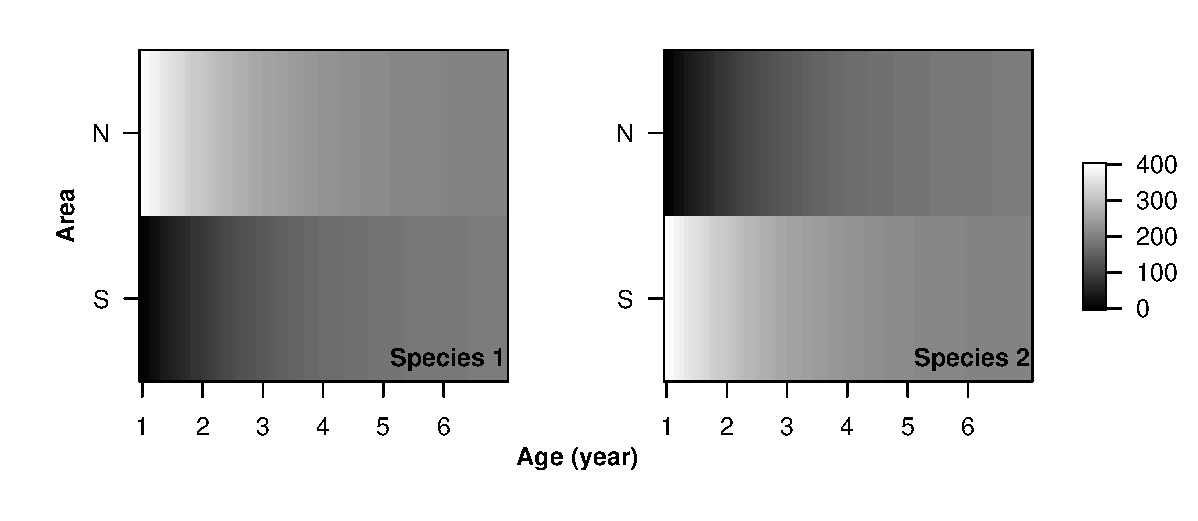
\includegraphics[width=.69\textwidth]{Figures/Distributions.eps} 
\caption{Distribution of the two species over the areas as a function of age when stocks are in virgin stock status }
\end{figure}
  
Age-dependent catchability linked the population biomasses to the catches in the fishery, and was thus one of the crucial parameters determining the interaction between the two. In the case study, this age-dependent catchability $q_i (a)$ was assumed independent of age $a$, and equal for the two species.

The mean prices for the two species were set to 30 thousand euro per ton, ranging between 29 thousand euro per ton for the youngest age and 30.5 thousand ton for the oldest age (Figure \ref{f:prices}). The fines for overshooting the quota was set  to 3000 thousand euro per ton (Table \ref{t:fishery}). These high fines combined with an assumed 100\% detection of exceeding quotas resulted in model results in which fishers comply with quota regulations.

\begin{figure}[!ht]
\centering
\label{f:prices}
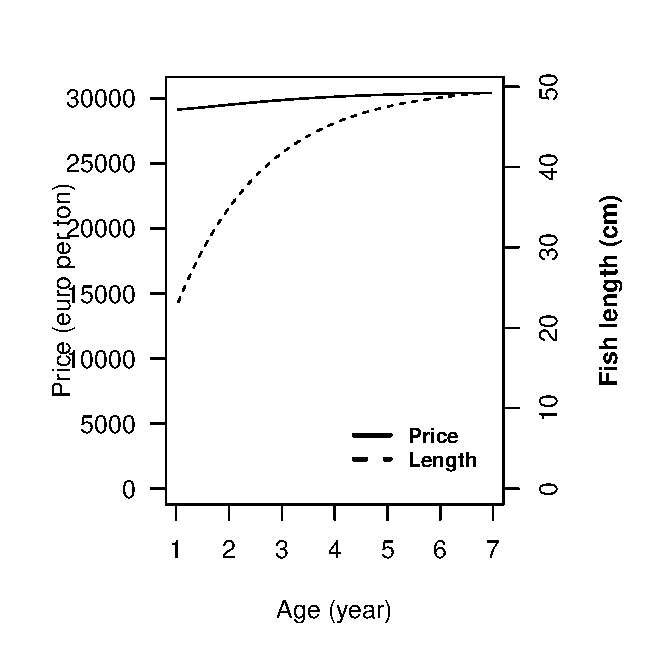
\includegraphics[width=.69\textwidth]{Figures/Prices.eps} 
\caption{Lengths and prices of the species}
\end{figure}

\subsection{Management procedure}

The input to the fisheries model consisted of the the expected catch rates and the individual quota that were set for each individual in the fleet. These individual quota were set in a management procedure, which mimicked the decisions of a management body. This management body made observations on the state of the resources, and the exploitation characteristics of the fishery. In the model, the management body was assumed to collect annual observations of the biomass of the stocks, including the distribution of the biomass over the different ages. These observations stem from fisheries independent observations, such as surveys with known catchabilities. In addition, the management body made annual observations of the catches, including their age distribution. The observed biomass and catches allowed for estimation of the annual harvest rates, and the estimation of a yield per recruit curve, that was dependent on fish growth and mortality. The yield curve was dome shaped, with a maximum that is called $H_{max}$. Fishing at a harvest rate that is equal to $H_{max}$  should lead to maximum sustainable yields. The yield per recruit curve omited the potential effect of the feedback between adult biomass and recruitment, which anyway was absent in the population dynamics, that assumed a constant recruitment. The Harvest Control Rule used by the management body resuslted in annual quotas such that the harvest rate in a year corresponded to $H_{max}$. These quotas were then divided equally over the individual vessels in the simulations.  




The management model encompassed the harvest control rules (HCR). The HCR referenced to biological reference points (Fmsy) to produce management actions in the form of a harvest or effort level: changes in selectivity or spatial and temporal reallocations or restrictions of fishing effort. Costs and benefits, both economic and in terms of risks to both stock and livelihoods, could be computed and compared across different scenarios and management procedures.

% Management actions are rarely implemented without error. This error can come from two main sourrces: (i) resource users do not comply with the regulations, and (ii) the individual dynamics of resource users (e.g. when and where harvest is taken) are not accounted for in the HCR. By evaluating a range of HCRs against a set of plausible operating models using multiple performance metrics (section \ref{sec2.3}), MSE enables to study the different trade-offs involved with each management procedure.  

\begin{equation}
 l_{ratio} (a, y, s) = \frac
                % Nominator
                {L_{i (numbers)}(a, y, s, p)}
                % Denominator
                {C_{i (numbers)}(a, y, s, p)},
\end{equation}

Through a yield per recruitment model, knowing growth, harvest rates and recruitment we can estimate how much to reduce the quota for achieving the MSY. 

\begin{equation}
 Q_{MSY} = \frac
                % Nominator
                {\sum( [\frac{H_{MSY}}{\bar{H}} \times H (a, s) \times l_{ratio} (a, s) \times B_{(numbers)}(a, s)] \times wts) }
                % Denominator
                {number\  of\  vessels}, 
\end{equation}
\begin{equation}
 Q (y+1) = \max( \min(Q_{MSY}, Q(y) \times 1.15), Q(y) \times 0.85), 
\end{equation}


%Given the landing parameters associated

%hr<- catches.n/ (catches.n+ pop)
%landings.ratio <- landings.n/ cathces.n
%OY <- 
%hr_MSY <- OY[OY_landings==max(OY_landingslandings),]_hr

%prel.quota <-  sum(sweep((hr1wanted[1]/mean(hr1[,yy,]))* hr1[,yy,]*landings.ratio1[,yy,]*apply(pop1[,yy+1,,],c(1,2), sum) ,1,wts,"*"))/SIMNUMBER
%        tac.constrained <- c(quota1[,yy,,]*0.85, quota1[,yy,,]*1.15)
%        quota1[,yy+1,,] <- max(min(prel.quota, tac.constrained[2]), tac.constrained[1])
        
        
%From an economic perspective, a linear increase towards maximum TAC is the optimal strategy under plausible assumptions on market demand for fish and harvesting cost, as shown in Froese et al., 2010. The economic rationale is that, beyond Blim, the stock is within safe biological limits, and as it becomes more and more productive, it is able to supply the market to an increasing extent. 

%A linear reduction in fishing mortality has been implemented in Australia (DAFF 2007) a nd is common in the USA. The differences between a linear decline in fishing mortality and a linear decline in TAC are small, see Figure A2 in Appendix S4.     

%estimating the hr Fisheries are managed by a total allowable catch (TAC). A maximum TAC is set for each stock so that the respective target biomass is maintained
%on average. This maximum TAC may be taken as long as biomass fluctuations remain above Bmsy. 


\subsection{Scenarios}

The model was set up in three consecutive time windows. In the first window of 10 years, newborns entered the population in the absence of fishing. This resulted in a virgin stock status. Then, the fleet of 8000 vessels started fishing in the absence of any fisheries regulations. This window lasted 15 years and gradually resulted in a situation where the stocks were overfished, i.e. the harvest rates were larger than $H_{max}$. Finally, the management procedure started where the HCR controls the annual quotas.  
      
The two management strategies we considered differ simply by the 


formulae used to determine exploitation rates (HCR). These management strategies were chosen such that, if  the  management  model  was  the  correct  model  of  reality,  the corresponding  equilibrium  state  of  the  system  would  meet  the  objective  of  the  plan. For this purpose, each strategy was implemented after a period where the fishery was unmanaged, by meaned with unconstrained quota for both species.

The comparison among these scenarios resulted in the 
However, the  long term benefits to fisheries that could result from improved selectivity are ignored in those studies. Ignoring the potential for improved selectivity leaves out a key element in the perceived benefit of the LO. Because the LO should provide incentives for the use of more selective gears and for fisheries to  move away from areas with high levels of unwanted catch \cite{Alzorriz2016, Alzorriz2018}, the improved selectivity should lead to higher long term catches. Achieving single species MSY while landing all commercial catches in fisheries targeting multiple species (mixed fisheries) is challenging because achieving the objective for one species may mean missing the objective for another \cite{Batsleer2013,Ulrich2017}. Forecasting whether such management will be effective depends on understanding the response of individual effort allocation to the management.

%\begin{table}[!h]
%\centering
%\caption{}
%\label{scenarios}
%\resizebox{0.8\textwidth}{!}{%
%\begin{tabular}{l c c}
%\hline
%                                & \textbf{MP}            & \textbf{LO}                  \\ 
%                                & \textit{(landings selectivity)}& \textit{(fulll avoidance of discards)}\\ \hline
%& &   \\
%Discarding                      & Allowed                        & Not allowed                 \\
%Manager catch perception        & $C = L + D$                    &        $C = L$ ($D = 0$)    \\
%Selectivity ($l_{ratio}$)       &  $ \neq 1$                     & $=1$                      \\
%Yield per recruitment model     & based in $F_L$                 &       based in $F_C$          \\

%&  &   \\\hline
%\end{tabular}
%}
%\end{table}
% 
%\begin{enumerate}

%\item
%\textbf{MP Scenario: Landings selectivity},  under this scenario the fishery is under landings selectivity, only landings contribute to yield. Fishing mortality accounts for all catches, regardless wether these catches are landed or discarded.

%\item
%\textbf{LO Scenario: Fulll avoidance of discards}, this scenario contemplates the LO with landings selectivity only and fulll avoidance of discards.


%\end{enumerate}



\section{Results}

We simulated the effects of implementing a Management Plan (MP) and the Landing Obligation (LO) without any exceptions or flexibility. To be able to analyse the results of this complex actions of implementing the MP and the LO, the implementations should start simultaneously for all stocks and fleets. Under the MP, the Harvest Control Rule for the TACs is to advise $F_{MSY}$ unless the biomass falls below a trigger biomass. If the biomass falls below this value, the advised TAC is based on the biomass trends. To check for trends, the latest biomass levels are compared to previous ones. If there is a decrease of a 20\% or more, the TAC is reduced by 15\%. If the comparision shows an increase of more then 20 \% the TAC is increased by 15\%.

\subsection{Catch decisions and location choice}

When discarding was allowed, but TACs changed by 15\% based on previous year but trying approximate to Fmsy, TACS showed a reduction and discards increased. 

The implementation of LO caused an increase in TACs and revenues were higher than when discarding was allowed. Some fishing opportunities are always lost under the landing obligation; the final fishing mortalities are lower than the target fishing mortalities (at least for one species). However, this does not necessarily imply that the catches will be lower with landing obligation than without it. Catches will be reduced in the initial years of landing obligation implementation. However, at Spawning stock biomass increases with LO, the catches will increase too. Although the fishing opportunities are lost due to the choke effect, the biomass of some stocks might increase; after a few years, this extra abundance could be converted into more catches. This implies that are fleets that, in the mid-term, could benefit from the landing obligation.

\begin{figure}[!ht]
\centering
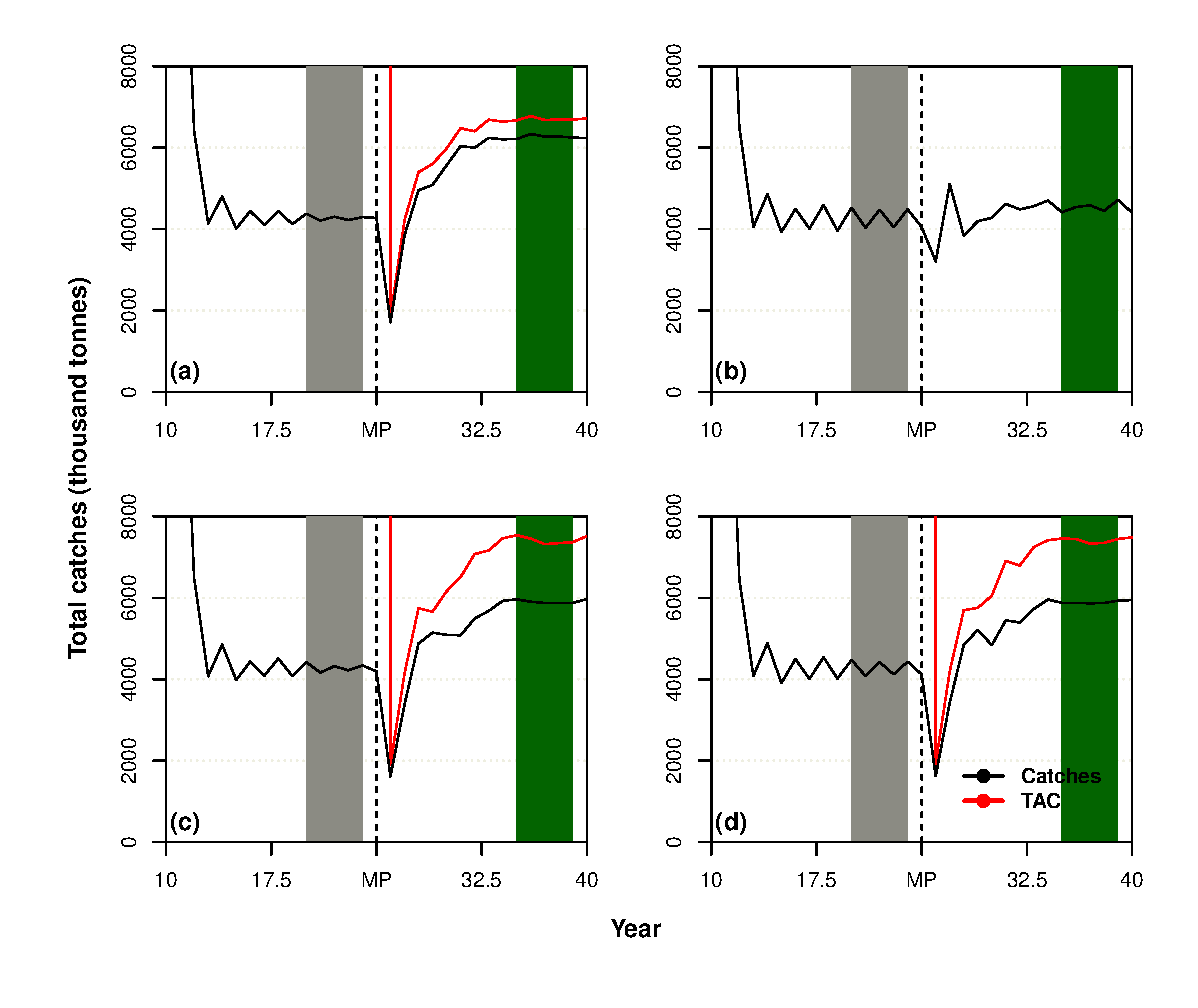
\includegraphics[width=\textwidth]{Figures/Catches.eps} 
\caption{Modelled total annual catches (thousand tonnes) for all vessels for both (a,c) species 1 and (b,d) species 2 in relation to the available individual quota (red line). In panels (a,b) only species 1 quota constrained the fishery, while in (c,d) both species quota constrained the fishery. MP year reflects the year where the management plan was introduced}
\end{figure}

\begin{figure}[!ht]
\centering
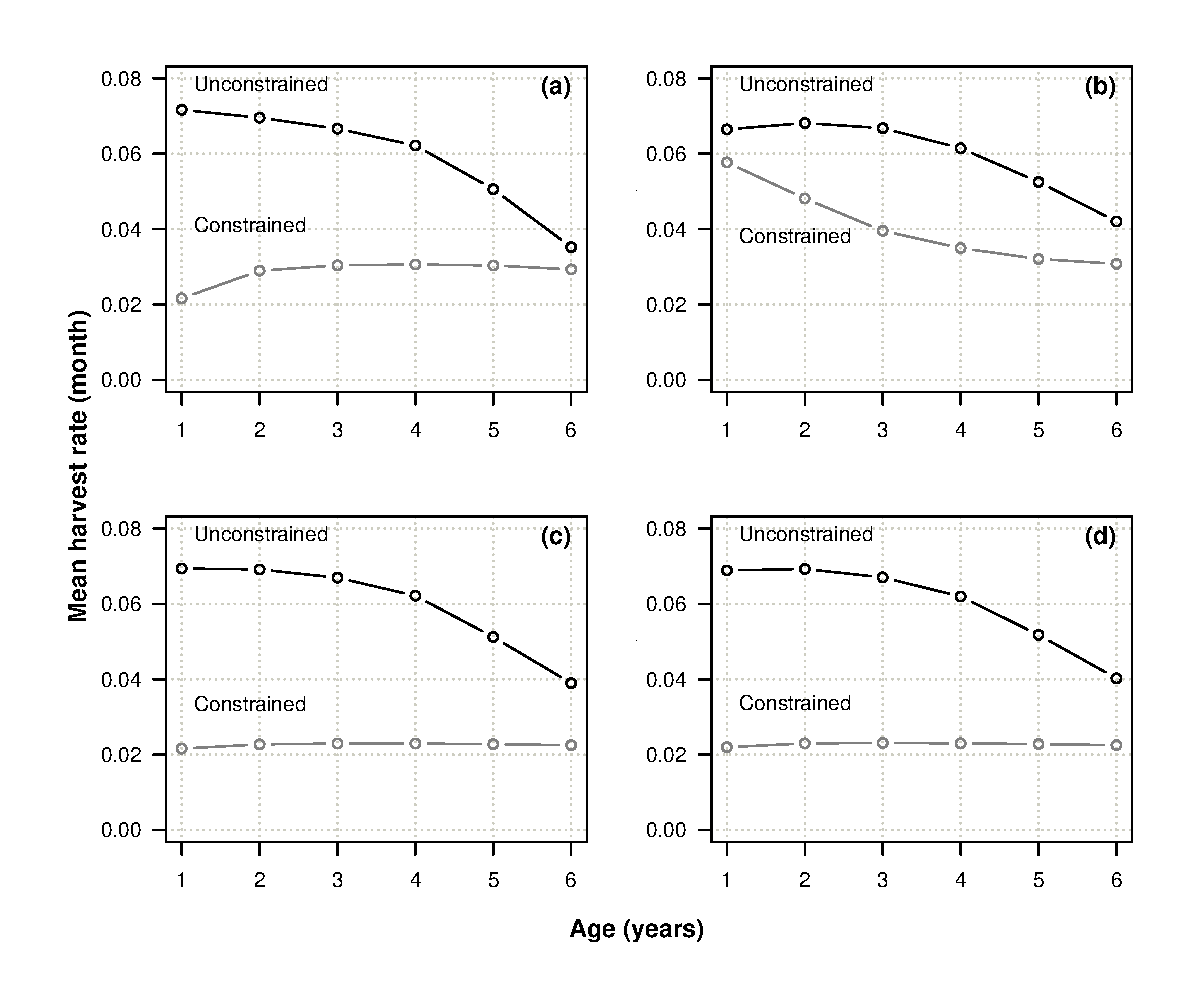
\includegraphics[width=\textwidth]{Figures/Selectivity.eps} 
\caption{Modelled changes in selectivity for both (a,c) species 1 and (b,d) species 2 in relation to the catch decision options made based in the availble individual quota. In panels (a,b) only species 1 quota constrained the fishery, while in (c,d) both species quota constrained the fishery. Black lines: selectivity curve before the MP period; grey line: selectivity curve after the introduction of the MP.}
\end{figure}

\begin{figure}[!ht]
\centering
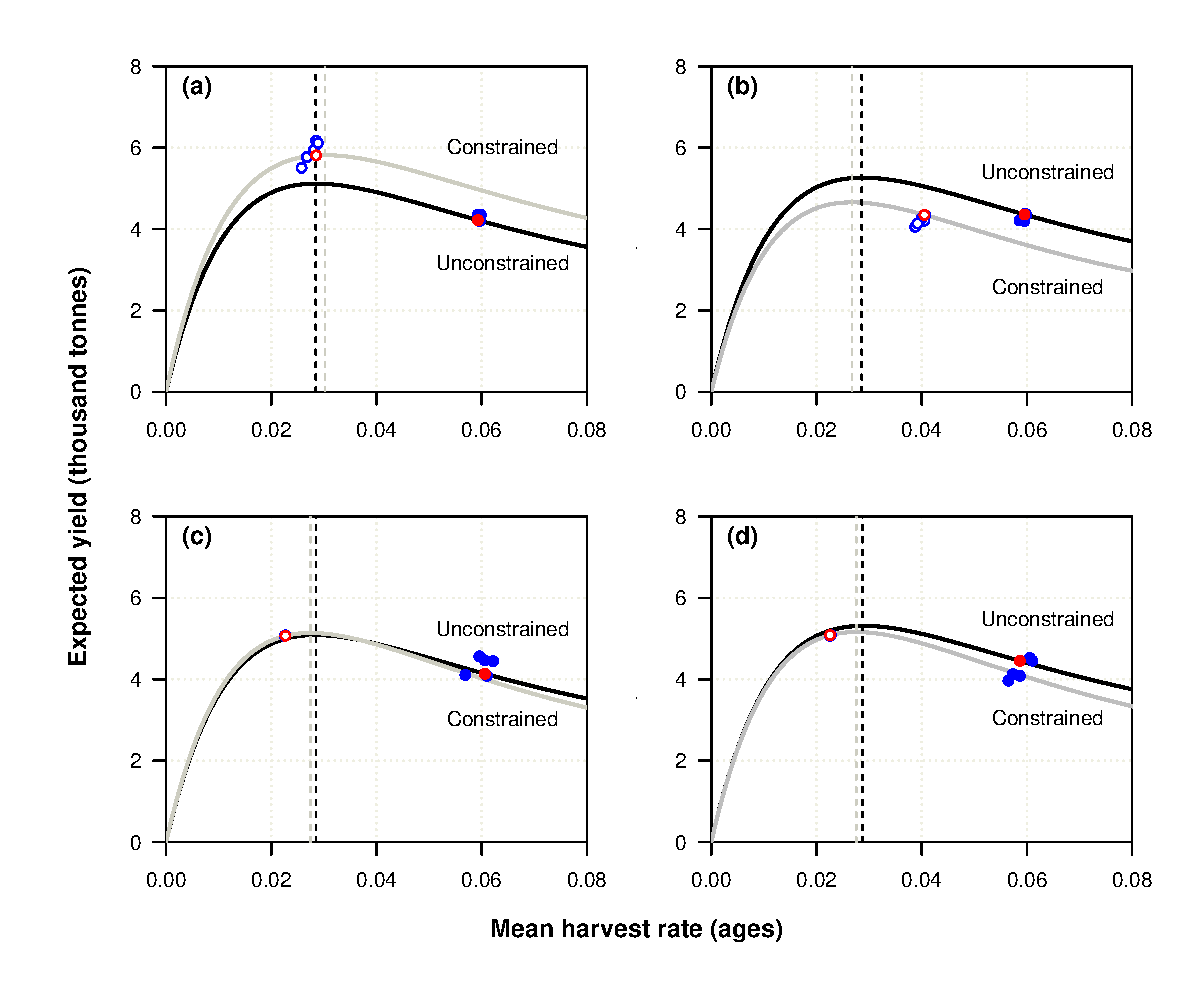
\includegraphics[width=\textwidth]{Figures/Yields.eps} 
\caption{Modelled yield per recruitment curves (thousand tonnes) for both (a,c) species 1 and (b,d) species 2 in relation to the management plan period (black line: period before the MP; grey line: period after the introduction of the MP). (a,c,d) After the introduction of the MP all species are underharvested to reach Fmsy, while in (b) species 2 is overharvested due to the abscence of any quota restriction.}
\end{figure}

\begin{figure}[!ht]
\centering
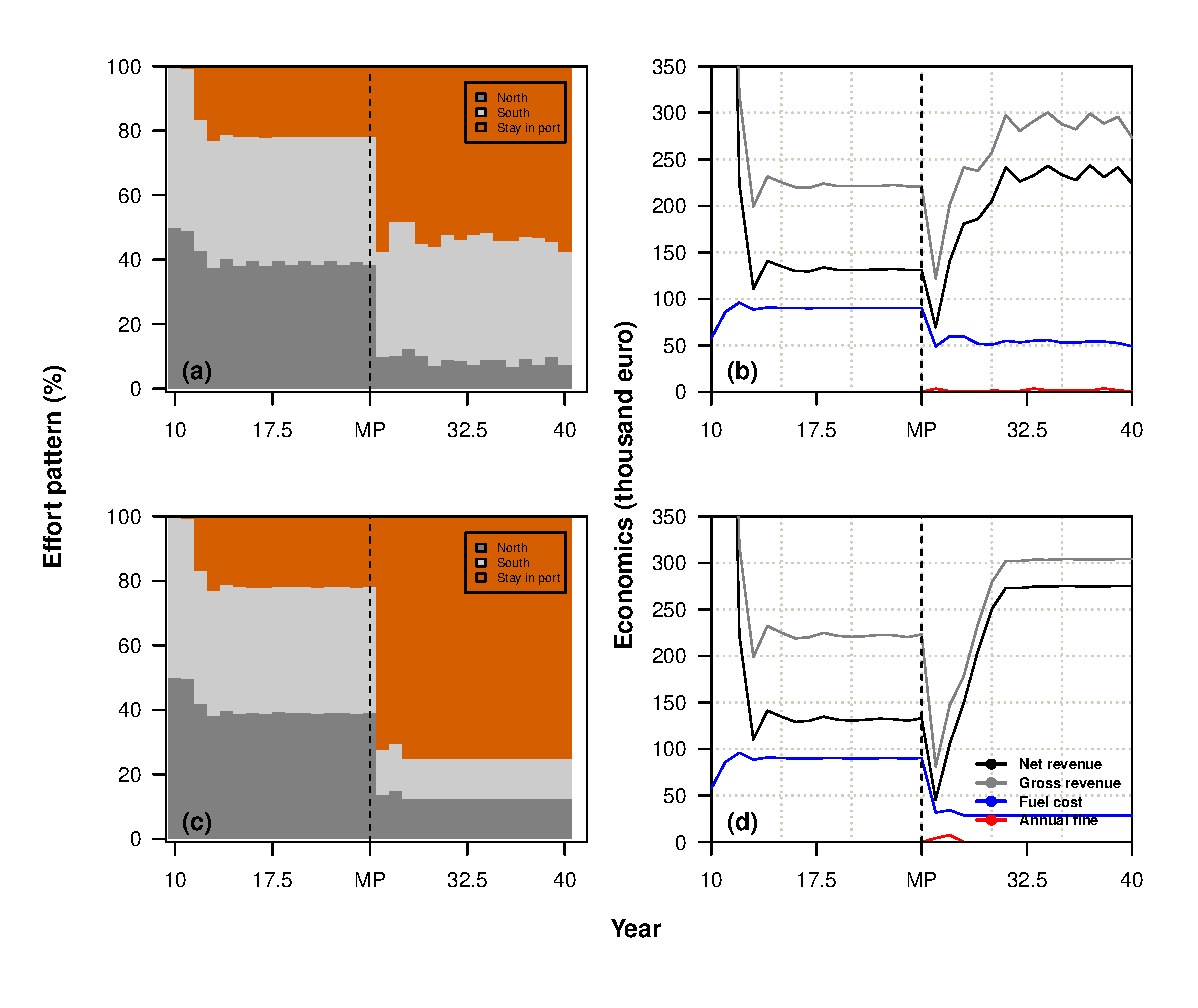
\includegraphics[width=\textwidth]{Figures/Efforteconomics.eps} 
\caption{Modelled spatial allocation of effort per year (\%) when (a) only species 1 has quota limitations and (d) both species are quota limited.  MP years reflect the year where the management plan was introduced. Panels (b-c) and (e-f) are the average monthly effort (days/month). Panels (b,e) are based on the 3 years monthly effort average (days) before the introduction of the MP, while (b,e) are the 3 years monthly effort average based on the period after the introduction of the MP.}
\end{figure}

\begin{figure}[!ht]
\centering
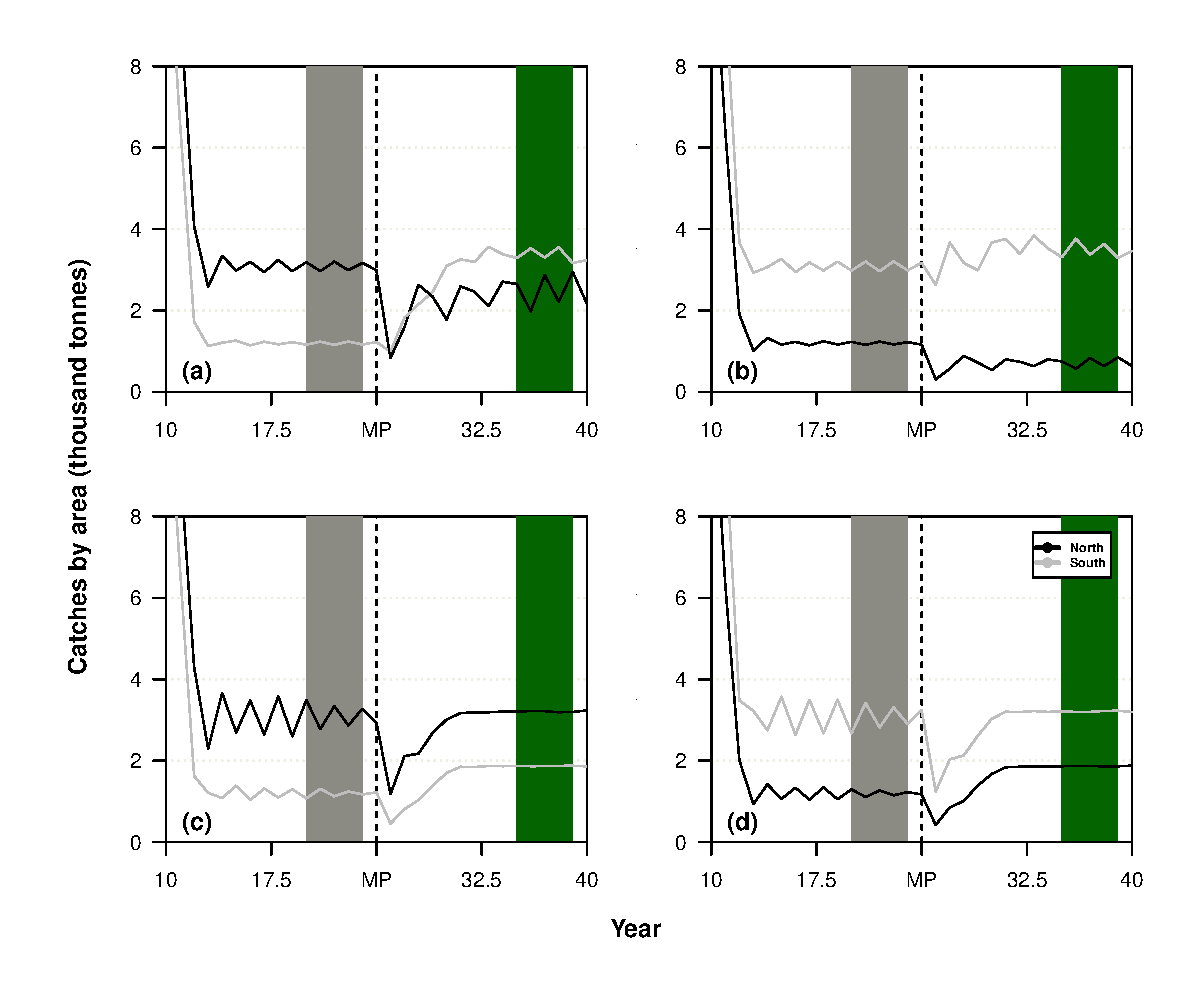
\includegraphics[width=\textwidth]{Figures/Catchesbyarea.eps} 
\caption{Modelled catches (thousand tonnes/year) by area (blue line: Northern area, red line: Southern area) for both (a,c) species 1 and (b,d) species 2 in relation to the management plan period. In panels (a,b) only species 1 quota constrained the fishery, while in (c,d) both species quota constrained the fishery. MP year reflects the year where the management plan was introduced.}
\end{figure} 

\begin{figure}[!ht]
\centering
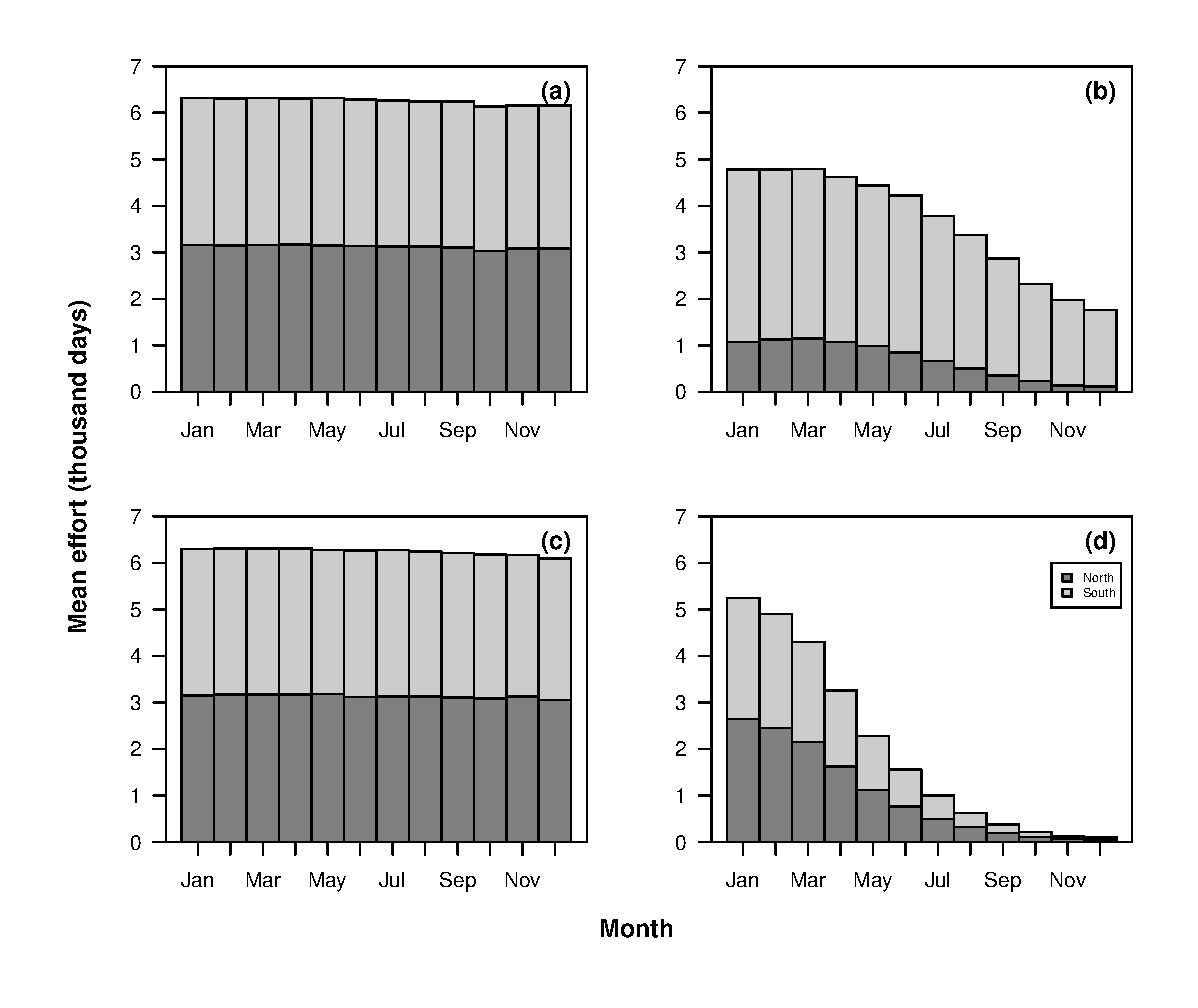
\includegraphics[width=\textwidth]{Figures/Meaneffort.eps} 
\caption{Modelled spatial allocation of effort per year (\%) when (a) only species 1 has quota limitations and (d) both species are quota limited.  MP years reflect the year where the management plan was introduced. Panels (b-c) and (e-f) are the average monthly effort (days/month). Panels (b,e) are based on the 3 years monthly effort average (days) before the introduction of the MP, while (b,e) are the 3 years monthly effort average based on the period after the introduction of the MP.}
\end{figure}

\begin{figure}[!ht]
\centering
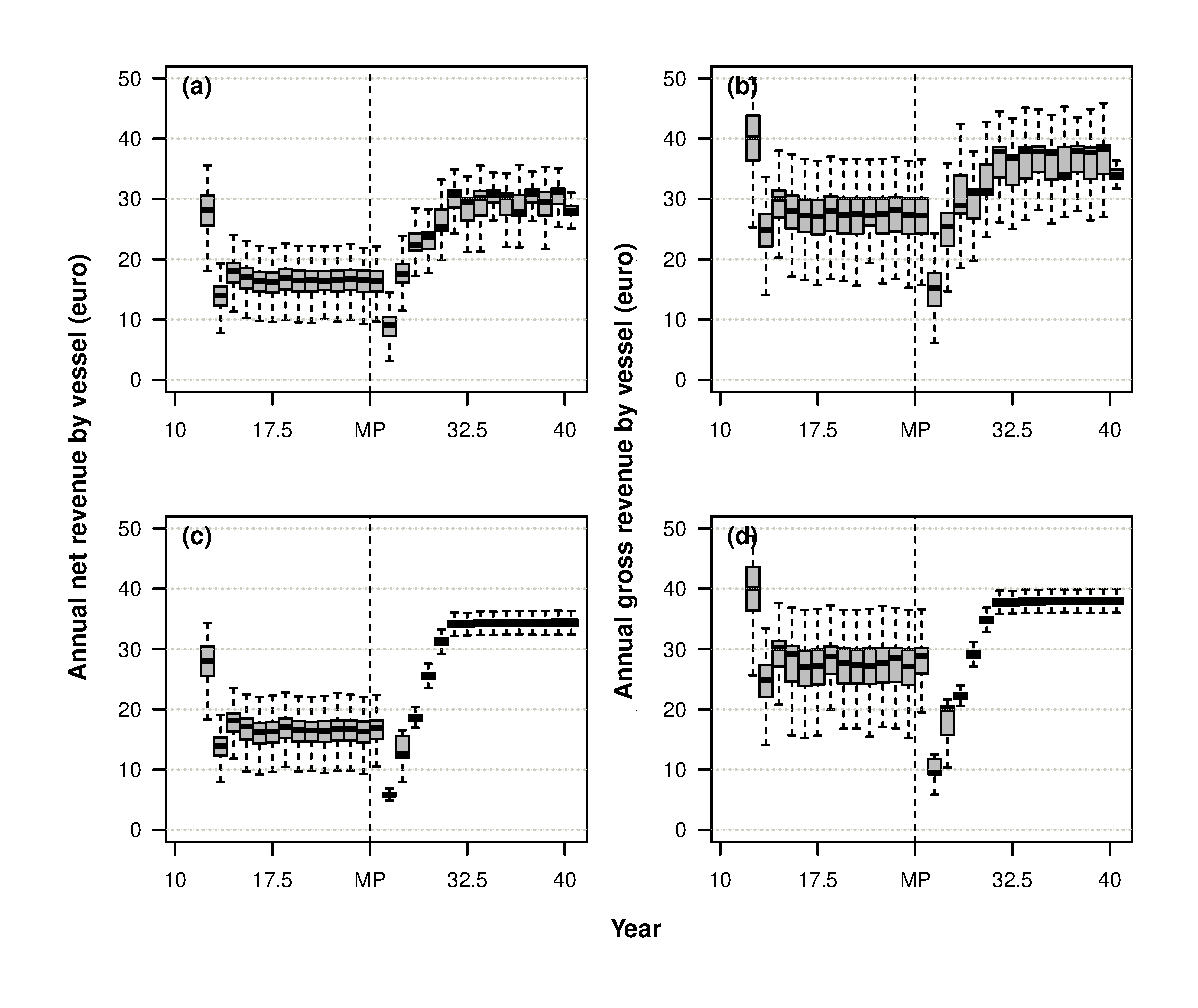
\includegraphics[width=\textwidth]{Figures/Mean_Economics.eps} 
\caption{Modelled main economics (thousand euro/ year) for the fleet under the management scenarios: (a-c) when the fishery is quota contrained only by species 1, while (d-f) both species constrained the fishery. Panels (a,d) and (b,e) shown the average annual net and grooss revenues, respectively, by vessel. MP year reflects the year where the management plan was introduced. Trade-offs between net revenue (black lline), gross revenue (grey line), fuel cost (blue line) and annual fines (red line) for the fleet are shown in panels (c,f).}
\end{figure}
%---

\clearpage

\section{Discussion}

tbd
prellezo 2016, In the mid-term and without any consideration made in terms of the ecosystem functioning as a whole, the results obtained from applying any kind of exemption or flexibility are, simply, negative. Fishing beyond FMSY (even in one year) implies that there will be a penalty in the future. This penalty will come in the form of lower biomasses, that has the mixed effect of increasing the cost of fishing the same level of catches and reducing the total catch due to the lower abundances and the subsequent lower TACs.

The largest yield (or catch) that can be taken from a species' stock over an indefinite period. Fundamental to the notion of sustainable harvest, the concept of MSY aims to maintain the population size at the point of maximum growth rate by harvesting the individuals that would normally be added to the population, allowing the population to continue to be productive indefinitely. Under the assumption of logistic growth, resource limitation does not constrain individuals’ reproductive rates when populations are small, but because there are few individuals, the overall yield is small. At intermediate population densities, also represented by half the carrying capacity, individuals are able to breed to their maximum rate. At this point, called the maximum sustainable yield, there is a surplus of individuals that can be harvested because growth of the population is at its maximum point due to the large number of reproducing individuals. Above this point, density dependent factors increasingly limit breeding until the population reaches carrying capacity. At this point, there are no surplus individuals to be harvested and yield drops to zero. The maximum sustainable yield is usually higher than the optimum sustainable yield and maximum economic yield

There is an extensive literature on fisheries economic theory in which the Gordon-Schaefer equilibrium production model is central (Gordon 1954, Schaefer 1957, Clark 1983). This theory holds that there is an economic TRP, the Maximum Economic Yield (MEY), which occurs at the effort level yielding the greatest margin of revenue over cost from the resource. 
For a linear cost curve, this inevitably occurs to the left of MSY on the fishing effort axis. Since Fmey occurs at lower levels of effort than Fmsy, the use of this economic Target Reference Point is less likely to result in biological overfishing than the use of Fmsy.

As a TRP, Fmey is responsive to any changes in the economic environment which affect either the value of fish, or the cost of fishing. It may also be dependent on changes in fish abundance, if market price increases with declining abundance and is independent of the availability of similar resources elsewhere. Subsidies or external economic considerations such as fuel taxes will also affect the location of an economic Reference Point (e.g. Panayotou 1988).

The effect of supply on fish prices may, under certain circumstances, result in higher total profit, or profit per unit catch, when total catch is reduced. This characteristic may be a consideration in setting target fishing levels or catches but is least likely to be effective in situations where fish prices are set by global markets, e.g. the tuna fishery for the canning industry.

The value of a unit weight of the landed catch may vary with the size of individual fish, and in multispecies fisheries with species composition. Both fish size and species composition are functions of fishing mortality, and based on purely economic criteria, may be used as target reference points. Even if the actual target F cannot be estimated, in theory, F could be adjusted in increments until the desirable target catch characteristics are achieved.

In considering TRPs based on economic criteria, it is important to be aware of the effect which the practice of discounting could have on reference points. In evaluating investment projects, including resource management, economists discount the future value of any commodity. Discount rates may be in the order of 10\%. In the case of a fishery where the population growth rate does not exceed the discount rate, then a strict application of economic theory would suggest that in the absence of other considerations (such as an economic value placed on recreational use of resources) the whole stock should be harvested now, and the proceeds of their sale invested. Long-lived species with slow growth rates, such as whales, clearly fall into this category. The blatant contradiction between this common economic approach, and the concept of sustainability, constitutes an unresolved paradox (Hilborn and Walters 1992).

\begin{notes}[Acknowledgements]
The content of this paper does not reflect the official opinion of the European Commission. Responsibility for the information and views expressed in this paper relies entirely with the authors.
\end{notes}


\bibliographystyle{plain}
\bibliography{mylib}



\end{document}
